\documentclass[11pt]{report}
\usepackage[utf8]{inputenc}
\usepackage[margin=2.0cm]{geometry}
\usepackage{tikz}
\usepackage{fancyhdr}
\usepackage{xcolor}
\usepackage{minted}
\usepackage{graphicx}
\usepackage[parfill]{parskip}
\usepackage{lscape}
\usepackage{multirow}

\usetikzlibrary{automata, positioning, arrows, fit}

\title{Digital Engineering\\Project Task 1}
\author{Y3890959\\Y3878784}
\date{28th February 2023}

\pagestyle{fancy}
\fancyhead{}
\setlength{\headheight}{14pt}
\fancyhead[L]{Project Task 1}
\fancyhead[R]{Y3890959, Y3878784}
\fancyfoot{}
\fancyfoot[L]{Digital Engineering}
\fancyfoot[R]{\thepage}

\makeatletter
\let\ps@plain\ps@fancy 
\makeatother

\setminted {
    fontsize=\footnotesize,
    frame=single,
}

\begin{document}

\maketitle

\chapter*{Task 1: Clock management through enable signals}

\section*{1 - FSM Description}

\begin{figure}[h] % ’ht’ tells LaTeX to place the figure ’here’ or at the top of the page
    \centering % centers the figure
    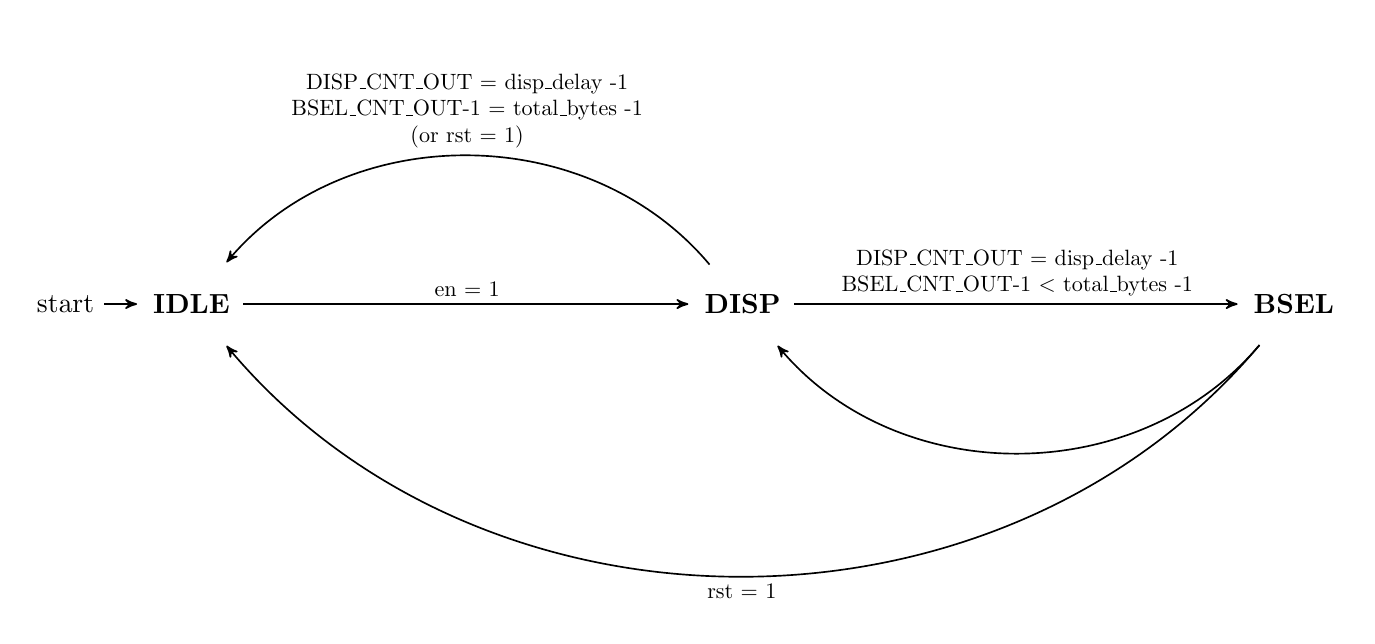
\begin{tikzpicture}[->,>=stealth',shorten >=1pt,auto,node distance=7cm,semithick]
        \tikzstyle{every state}=[draw=none,text=black]

        \node[initial,state] (A)              {\textbf{IDLE}};;
        \node[state]         (B) [right of=A] {\textbf{DISP}};
        \node[state]         (C) [right of=B] {\textbf{BSEL}};

        \path (A) edge                         node[scale=0.8] {en = 1} (B)
              (B) edge                         node[align=center, scale=0.8] {DISP\_CNT\_OUT $=$ disp\_delay -1\\BSEL\_CNT\_OUT-1 $<$ total\_bytes -1} (C)
                  edge [above, bend right=50]  node[align=center, scale=0.8] {DISP\_CNT\_OUT $=$ disp\_delay -1\\BSEL\_CNT\_OUT-1 $=$ total\_bytes -1\\(or rst = 1)} (A)
              (C) edge [below, bend left=50]   (B)
                  edge [below, bend left=50]   node[scale=0.8] {rst = 1} (A);
    \end{tikzpicture}
    \caption{FSM state graph}
    \label{fig:my_label}
\end{figure}

Abbreviations: DISP\_CNT - the counter that adds a delay to the LED display output. BSEL\_CNT - the counter
that increments for BSEL (byte select) so the correct byte can be displayed.

The FSM starts at IDLE state, where `EN\_SOURCE' is low, all internal counters (BSEL and DISP) are reset and
the LED array is off. When the `en' pushbutton is toggled, the DISP state is entered. Entering this state
after IDLE, the counters will be at 0, therefore `EN\_SOURCE' will be set high, then low as soon as either of
the counters start incrementing. This will trigger `DATA\_SOURCE' to compute the next value which will be
displayed. The DISP counter will start incrementing to add a delay for the LED display, once the counter
reaches a maximum and the BSEL counter hasn't yet reached a maximum, the BSEL state will be set. Otherwise,
the FSM goes back to the IDLE state as all bytes have been displayed with the delay. In the BSEL state, the
DISP counter is reset and disabled, and the BSEL counter is enabled for an increment. Going back to DISP state
will reset the BSEL counter. When the `rst' button is toggled at any point, the logic must reset to IDLE.

\newpage
\begin{landscape}
    \begin{table}
    \centering
    \resizebox{\columnwidth}{!}{%
    \begin{tabular}{|l|l|l|l|l|l|l|}
    \hline
    \textbf{STATE} &
      \textit{\textbf{EN\_SOURCE}} &
      \textit{\textbf{DISP\_CNT\_EN}} &
      \textit{\textbf{DISP\_CNT\_RST}} &
      \textit{\textbf{BSEL\_CNT\_EN}} &
      \textit{\textbf{BSEL\_CNT\_RST}} &
      \textit{\textbf{LED\_DISPLAY}} \\ \hline
    IDLE & 0                            & 0 & 1 & 0 & 1 & 00000000                                                                                    \\ \hline
    \multirow{4}{*}{DISP} &
      \multirow{2}{*}{\begin{tabular}[c]{@{}l@{}}1 when DISP\_CNT\_OUT \\ and DISP\_CNT\_OUT = 0\end{tabular}} &
      \multirow{4}{*}{1} &
      \multirow{4}{*}{0} &
      \multirow{4}{*}{0} &
      \multirow{4}{*}{0} &
      \begin{tabular}[c]{@{}l@{}}SOURCE\_DATA{[}7:0{]}\\ when DISP\_CNT\_OUT is 0\end{tabular} \\ \cline{7-7} 
         &                              &   &   &   &   & \begin{tabular}[c]{@{}l@{}}SOURCE\_DATA{[}15:8{]}\\ when DISP\_CNT\_OUT is 1\end{tabular}  \\ \cline{2-2} \cline{7-7} 
         & \multirow{2}{*}{0 otherwise} &   &   &   &   & \begin{tabular}[c]{@{}l@{}}SOURCE\_DATA{[}23:16{]}\\ when DISP\_CNT\_OUT is 2\end{tabular} \\ \cline{7-7} 
         &                              &   &   &   &   & \begin{tabular}[c]{@{}l@{}}SOURCE\_DATA{[}31:24{]}\\ when DISP\_CNT\_OUT is 3\end{tabular} \\ \hline
    BSEL & 0                            & 0 & 1 & 1 & 0 & 00000000                                                                                    \\ \hline
    \end{tabular}%
    }
    \caption{FSM table of outputs}
\end{table}
\end{landscape}
\newpage

\section*{2 - VHDL Code for `STUDENT\_AREA'}
\inputminted{vhdl}{../../../DE_Project_T1/DE_Project_T1.srcs/sources_1/imports/DigEng_Proj_T1_model/STUDENT_AREA.vhd}

\newpage

\section*{3 - VHDL Testbench}
\inputminted{vhdl}{../../../DE_Project_T1/DE_Project_T1.srcs/sim_1/imports/DigEng_Proj_T1_model/TOP_LEVEL_tb.vhd}

\newpage

\section*{4 - Behavioural Simulation Waveforms}

\subsection*{Global Reset and Initialisation}
\begin{figure}[H]
    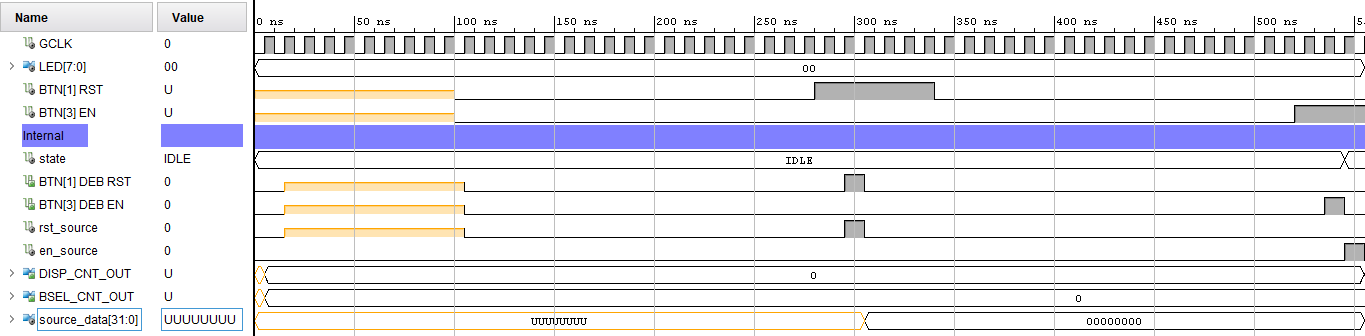
\includegraphics[width=\columnwidth]{Assets/reset.png}
\end{figure}
The above waveform shows a global reset, verifying that the circuit can be reset with the `rst' pushbutton.

\subsection*{Test 1, Waveform 1}
\begin{figure}[H]
    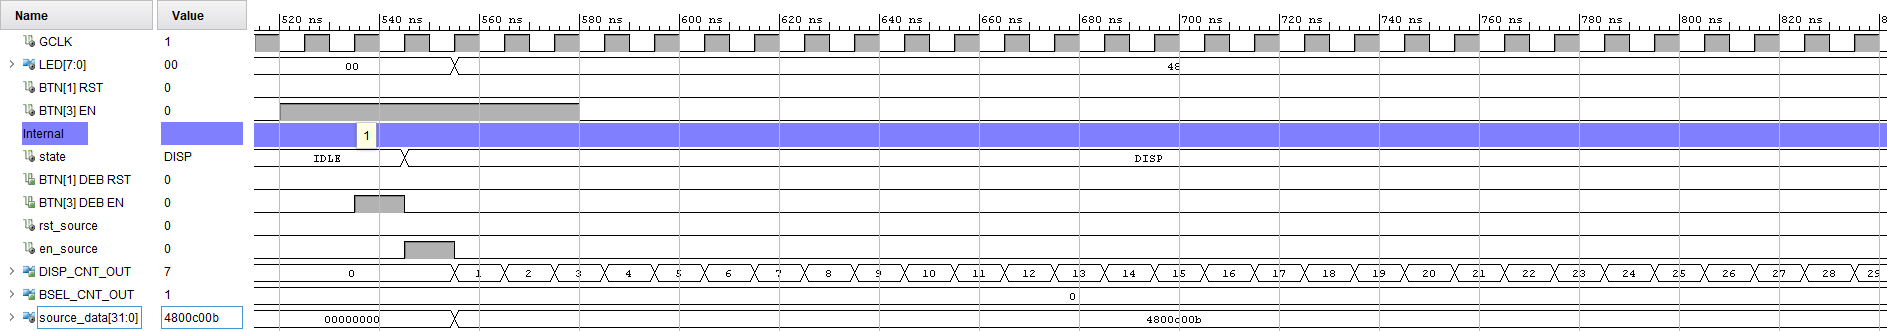
\includegraphics[width=\columnwidth]{Assets/test1_1.png}
\end{figure}
The above waveform shows an initial `en' toggle, followed by the output being computer and the first byte
being displayed on to the LED, it also verifies that the BSEL counter is fixed with the DISP counting.

\subsection*{Test 1, Waveform 2}
\begin{figure}[H]
    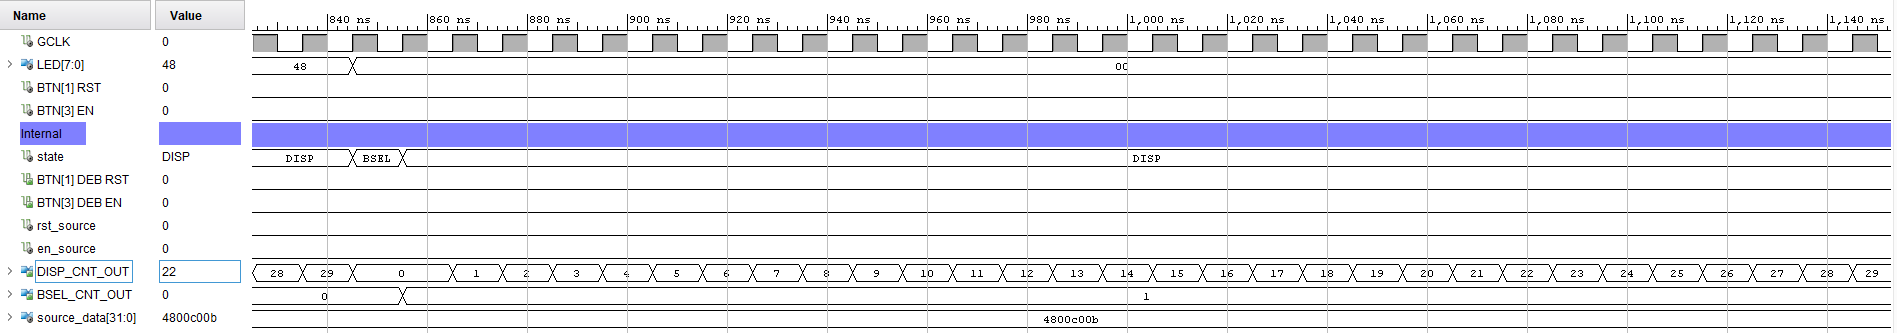
\includegraphics[width=\columnwidth]{Assets/test1_2.png}
\end{figure}
This waveform verifies that the DISP counter rolls over correctly, the BSEL increments and the LED is
displaying the correct (2nd) byte of the computed output

\subsection*{Test 1, Waveform 3}
\begin{figure}[H]
    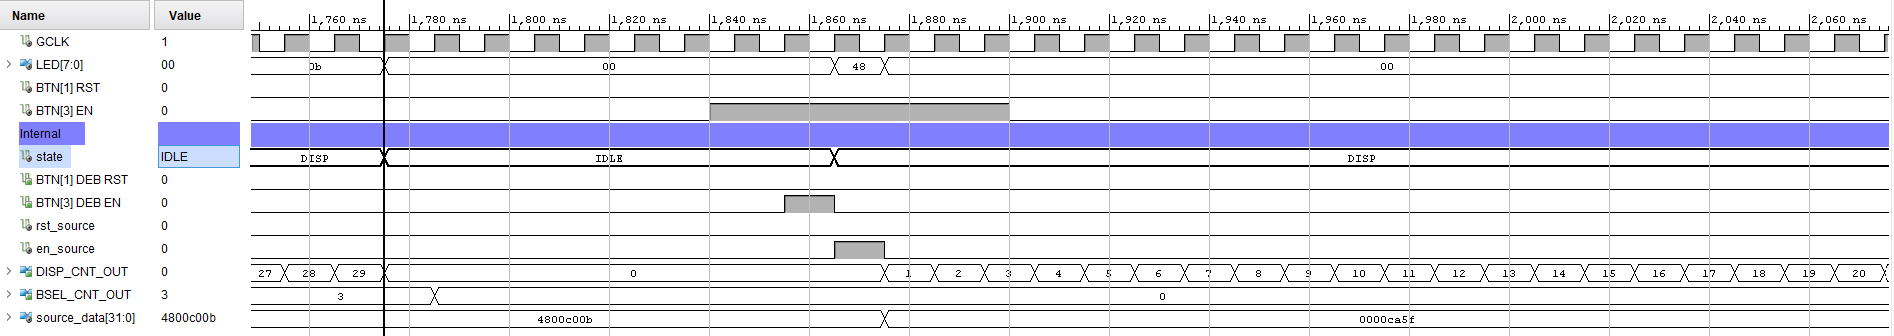
\includegraphics[width=\columnwidth]{Assets/test1_3.png}
\end{figure}
This waveform verifies the logic of finishing displaying the 4 bytes with a display delay and setting the
next state to IDLE. It also verifies that the `en' pushbutton can be pressed again to make the logic display
the next computed output.

\subsection*{Test 1, Waveform 4}
\begin{figure}[H]
    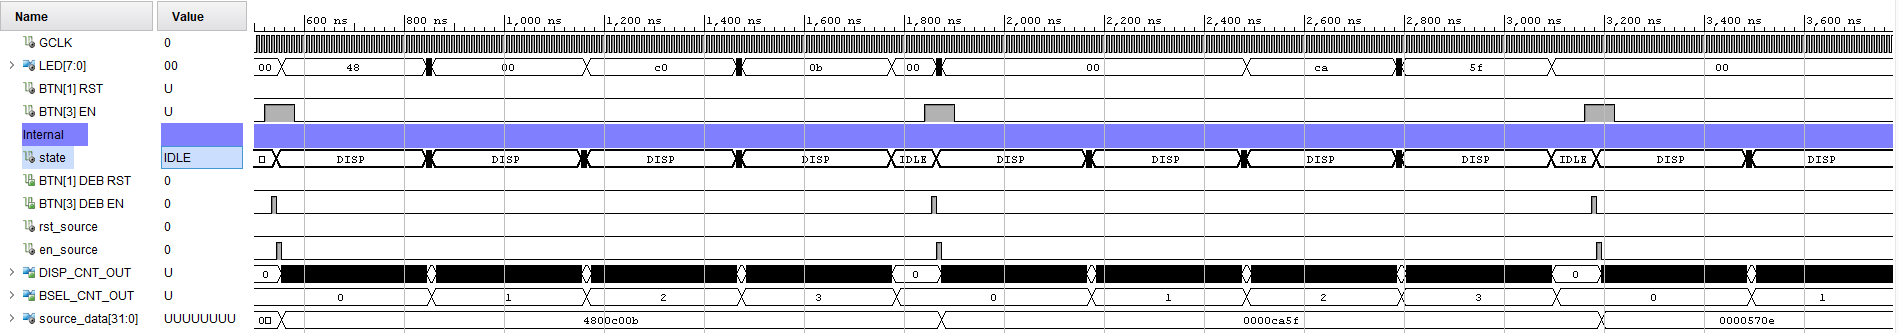
\includegraphics[width=\columnwidth]{Assets/test1_4.png}
\end{figure}
A very zoomed out waveform that verifies the logic as a whole: looking at the first three enable toggles,
the correct values are computed, the delays are working perfectly, the byte select is also working as intended
with the LEDs displaying the correct output.

\subsection*{Test 2}
\begin{figure}[H]
    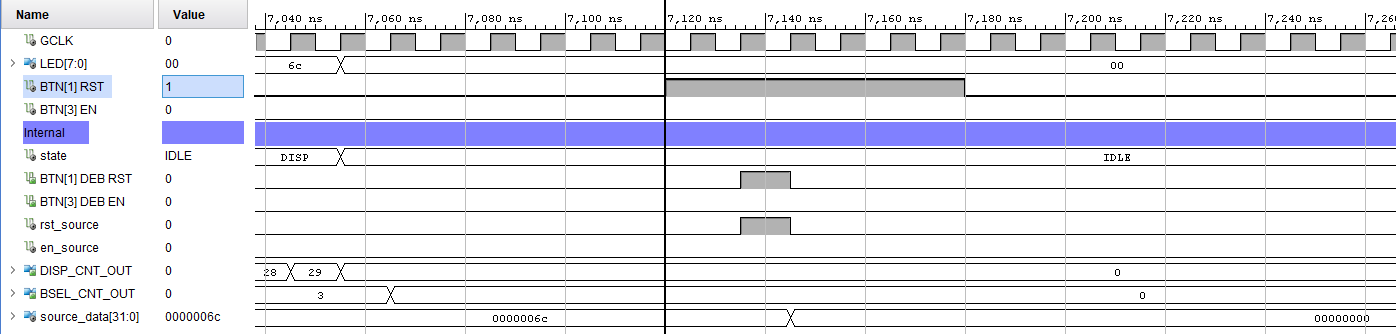
\includegraphics[width=\columnwidth]{Assets/test2.png}
\end{figure}
Following from Test 1, Test 2 consists of a `rst' toggle to verify that the logic can reset sucessfully. As
the waveform shows, this works as intended.

\subsection*{Test 3}
\begin{figure}[H]
    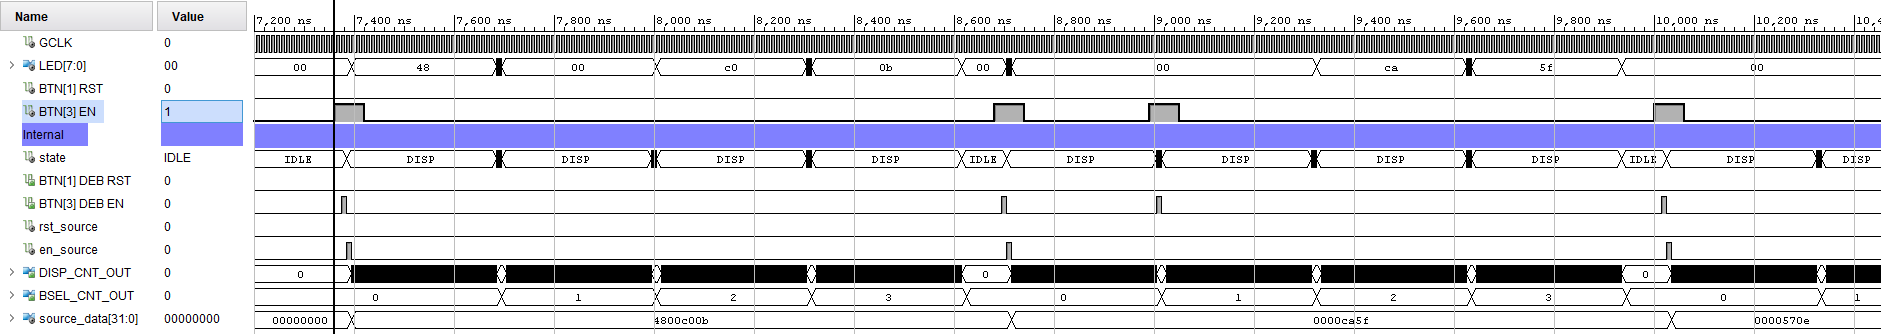
\includegraphics[width=\columnwidth]{Assets/test3.png}
\end{figure}
Another very zoomed out waveform which simply verifies that the logic ignores an `en' toggle when in any state
other that IDLE. When the `en' button is toggled at around 9000ns, the circuit is in DISP and BSEL
(shown as the black box due to being zoomed out). The logic sucessfully ignores it and carries on computing and
displaying the next values.

\subsection*{Test 4}
\begin{figure}[H]
    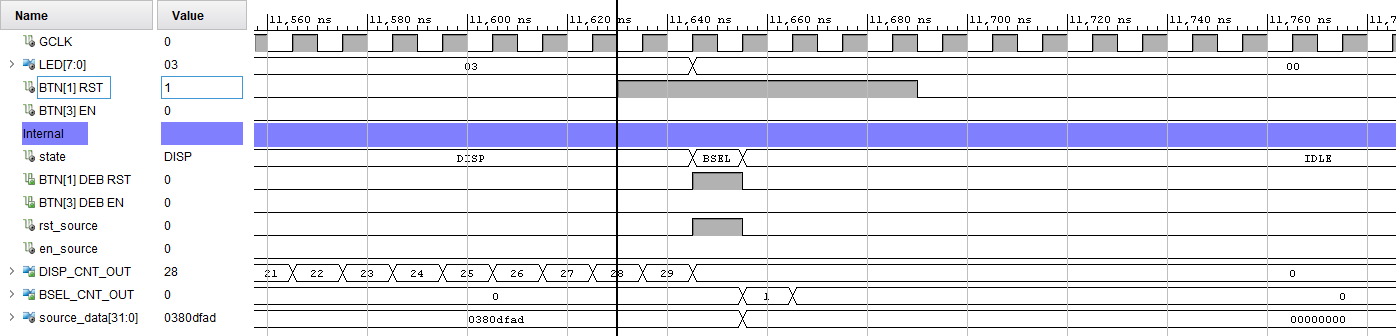
\includegraphics[width=\columnwidth]{Assets/test4.png}
\end{figure}
This test verifies that the circuit can be reset whilst the FSM is in operation. The logic successfully resets
back to the IDLE state with all internal signals and counters reset too. The circuit is now ready to continue
operation once the user toggles `en'. 

\newpage
\section*{5 - Synthesis Report}
\subsection*{RTL Component Statistics}
\inputminted[firstline=128,lastline=151]{text}{../../../DE_Project_T1/DE_Project_T1.runs/synth_1/TOP_LEVEL.vds}
\newpage
\subsection*{RTL Hierarchical Component Statistics}
\inputminted[firstline=154,lastline=208]{text}{../../../DE_Project_T1/DE_Project_T1.runs/synth_1/TOP_LEVEL.vds}

\end{document}
